\clearpage
\section{Cow Protocol}

\begin{refsection}

\begin{tcolorbox}	
\begin{tabular}{p{2.75cm} p{0.2cm} p{10.5cm}} 	
\textbf{Student Name}  &:&  Jo\~ao Ant\'onio\\
\textbf{}  & &  Daniel Pereira\\
\textbf{Goal}          &:& Explain the Coherent One Way (COW) Protocol and test it's strength against a intercept resend attack.\\
\textbf{Directory}              &:& sdf/tq_76558_cow_protocol
\end{tabular}
\end{tcolorbox}

The Coherent One Way (COW) protocol is one Quantum Key Distribution (QKD) what uses Time Bin properties, a simple scheme can be seen in the figure \ref{fig:Scheme}.

\begin{figure}[h]
\centering
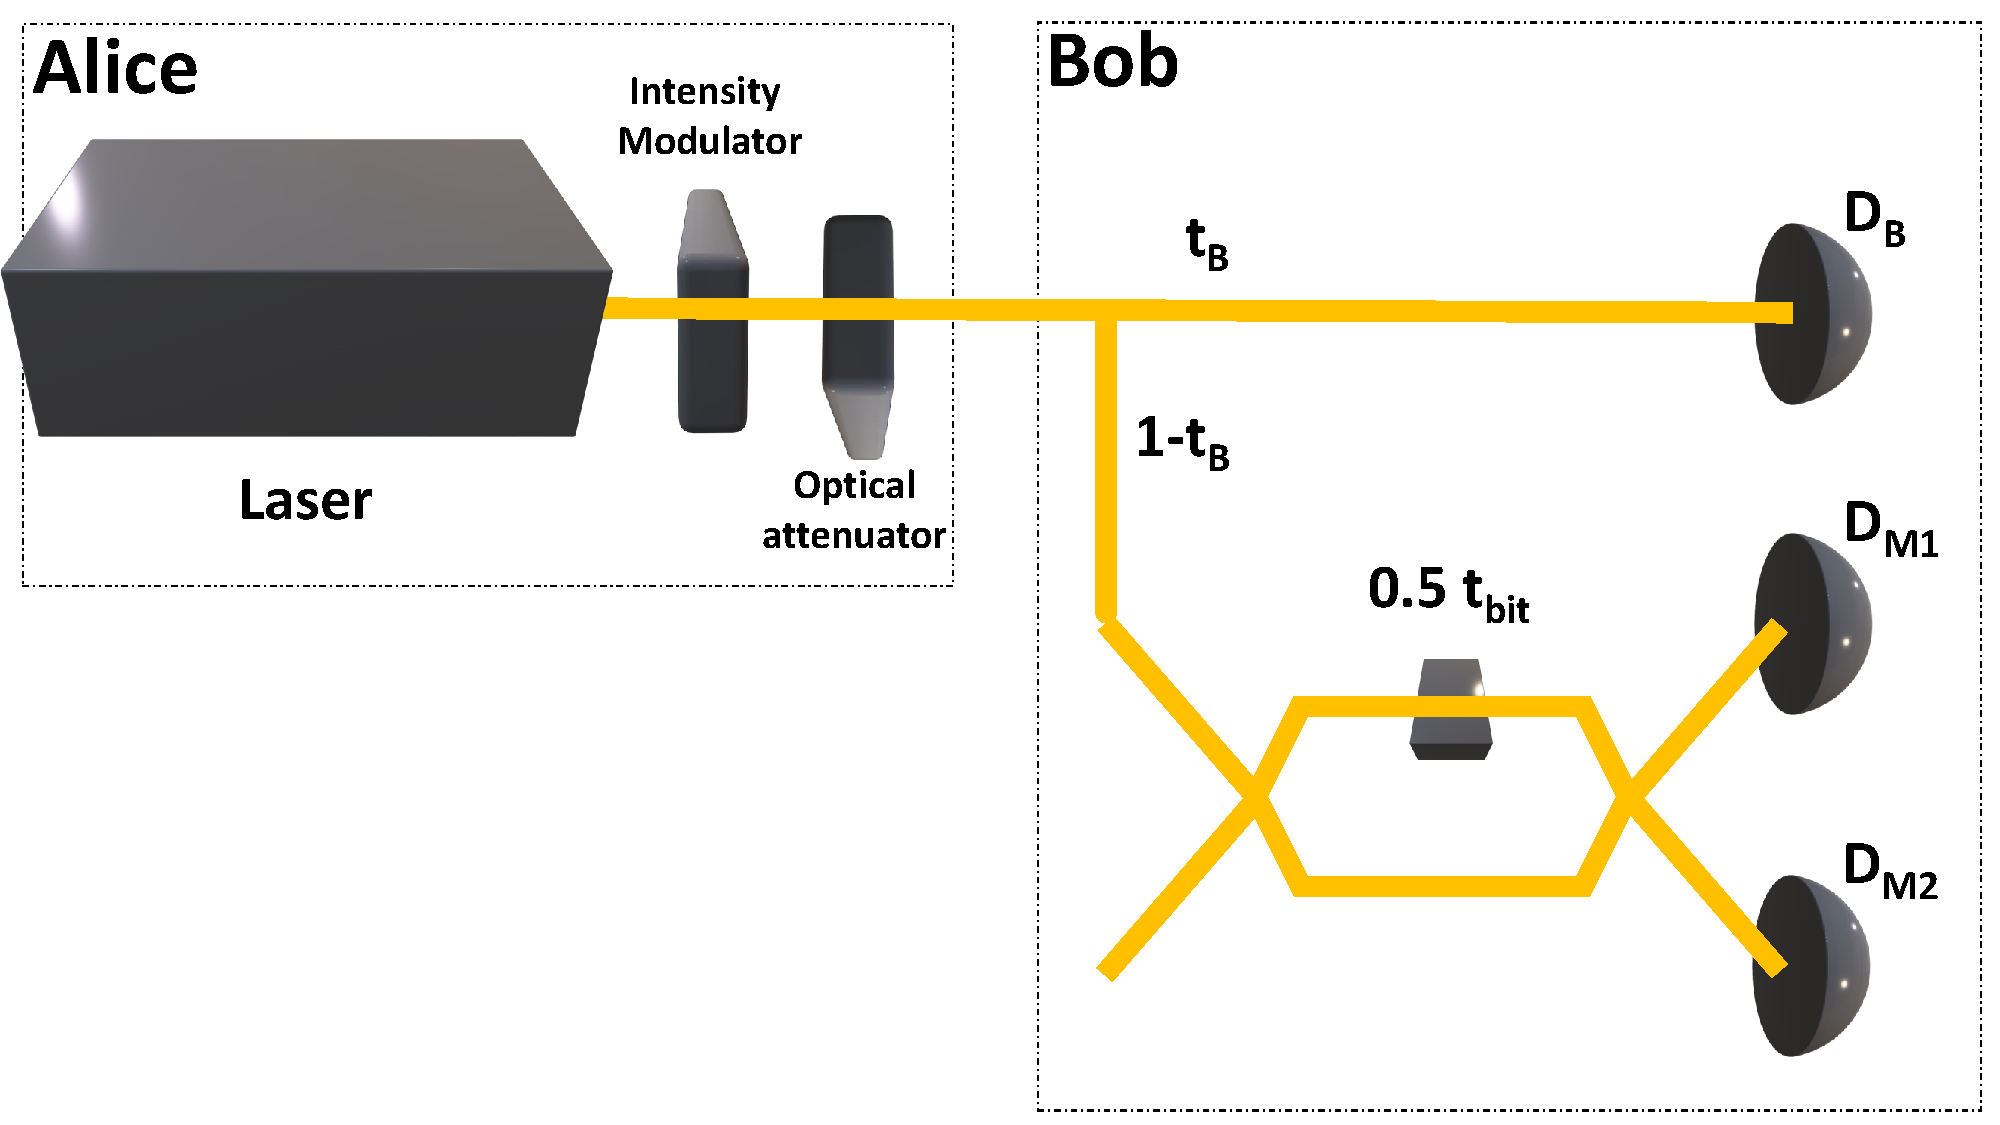
\includegraphics[width=.4\linewidth]{./sdf/tq_76558_cow_protocol/slides/figures/Full2.pdf}
\caption{Simple Scheme of the Protocol.}
\label{fig:Scheme}
\end{figure}

\par
It was created by Nicolas Gisin et al in 2004, and comparatively to the BB84 protocol has a much simpler set-up, since the Bob apparatus is passive, i.e. doesn't need to change basis, or anything actually.
\par
The purpose of this protocol is to create a secure key using quantum proprieties, just like any other QKD.

\subsection{Theoretical Analysis}

\begin{itemize}
\item [Step 1] Alice creates a random key using:
$$|0\rangle = |\alpha\rangle |\emptyset\rangle =\ \ Logical\ 0\ $$
  $$|1\rangle = |\emptyset\rangle |\alpha\rangle =\ \ Logical\ 1\ $$
$$|d\rangle = |\alpha\rangle |\alpha\rangle = Decoy State$$

Where $|\emptyset\rangle$ is the vacuum state and $|\alpha\rangle$ is a coherent state of light with intensity $\mu=|\alpha|^2<<1$. This can be seen in figure \ref{fig:sta}.
The probability of creating a |0\rangle state and a |1\rangle is equal, the probability of creating a |d\rangle state is usually 10 \%, while the attenuation value is usually 0.1.

\begin{figure}[h]
\centering
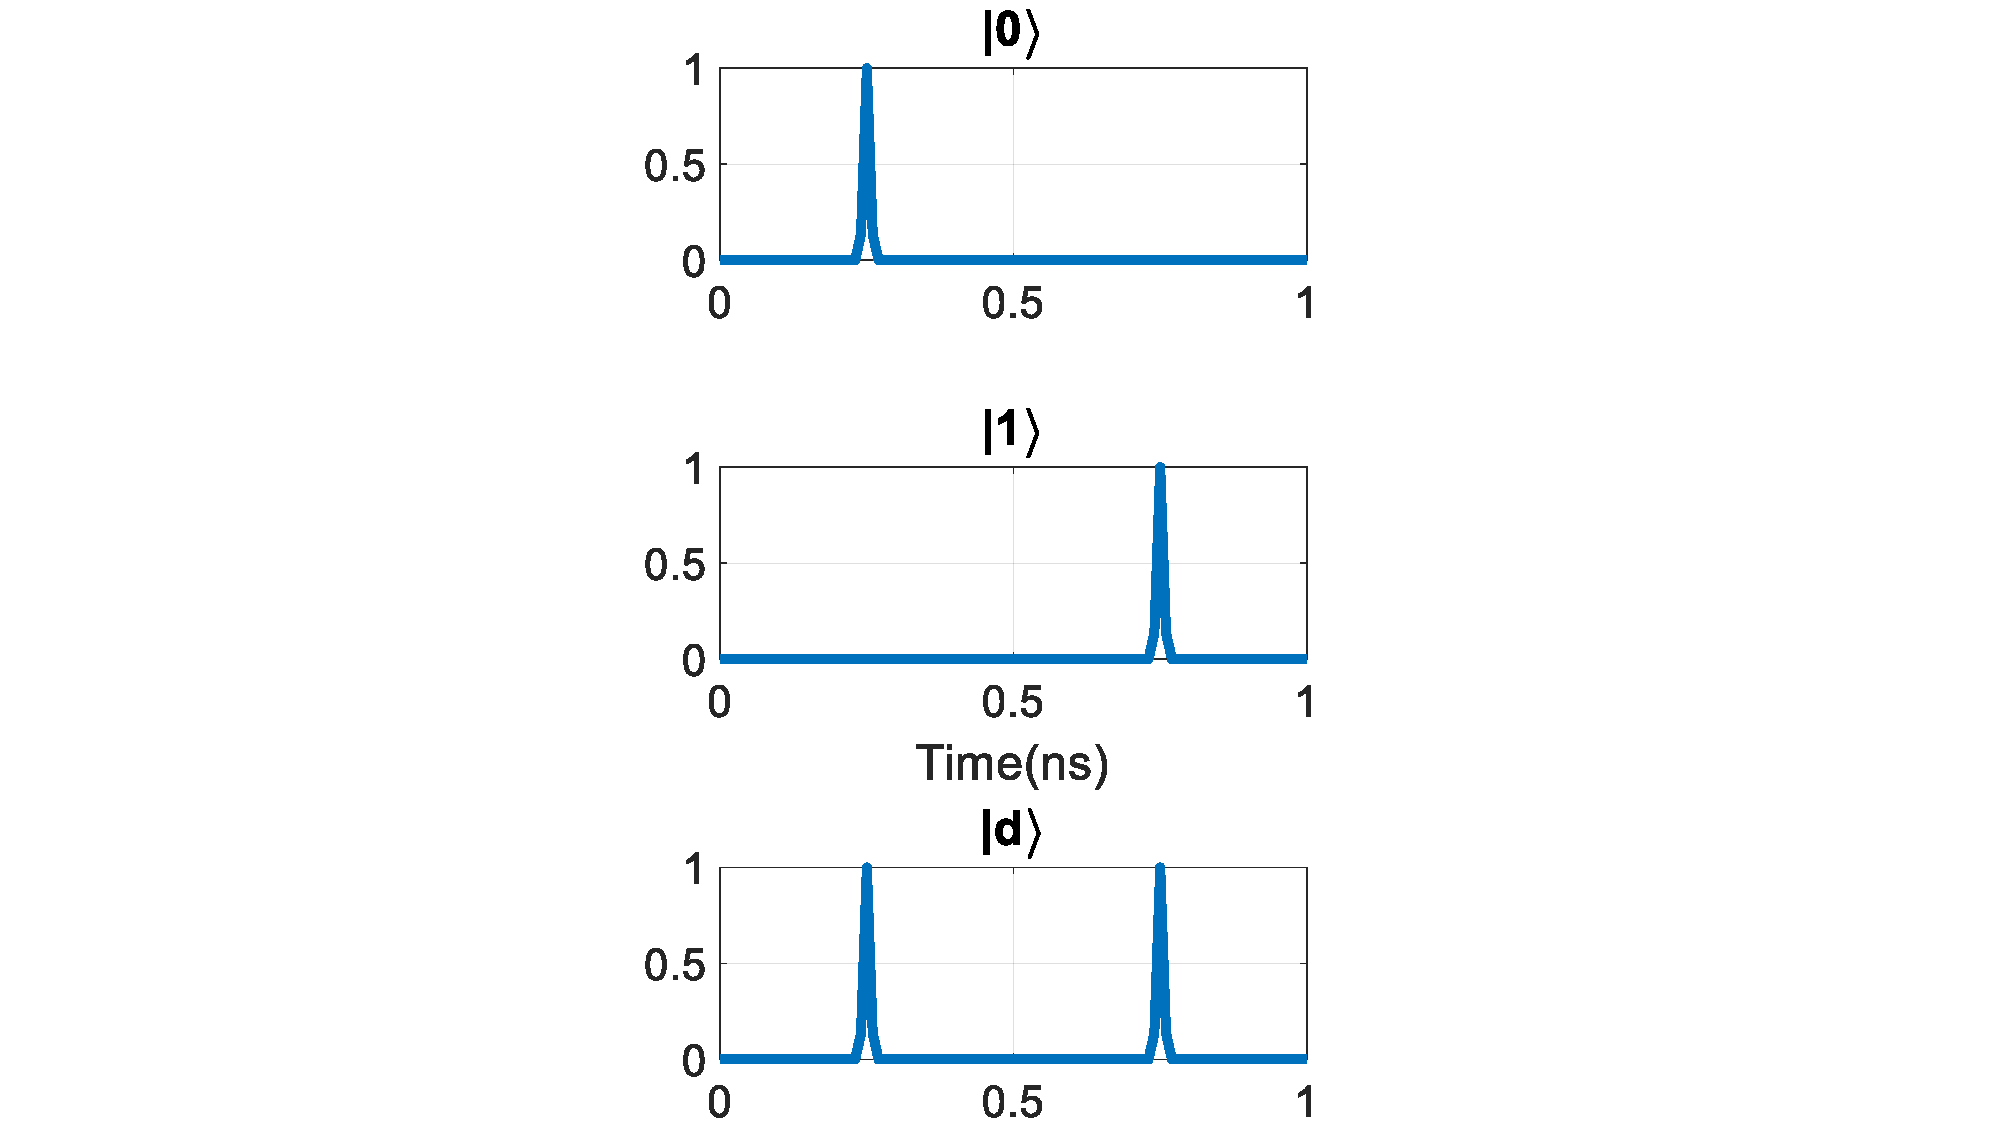
\includegraphics[width=0.4\linewidth]{./sdf/tq_76558_cow_protocol/slides/figures/S1A.pdf}
\caption{Representation of the states.}
\label{fig:sta}
\end{figure}

\item [Step 2]  In the Bob apparatus : a fraction $t_B$ of the photons go into the photon counter $D_B$, where the bits are discriminated by the time of arrival, usually 90 \%, while the rest go in to the monitoring line.

In this monitoring line, the photons have a 50 \% probability of being delayed by 0.5 $t_{bit}$ interacting with the non-delayed photons.

Therefore $D_{M2}$ (constructive photon counter) should only click in the |d\rangle state or in the |1\rangle state followed by the |0\rangle state, also represent in the figure \ref{fig:dm2}

\begin{figure}[h]
\centering
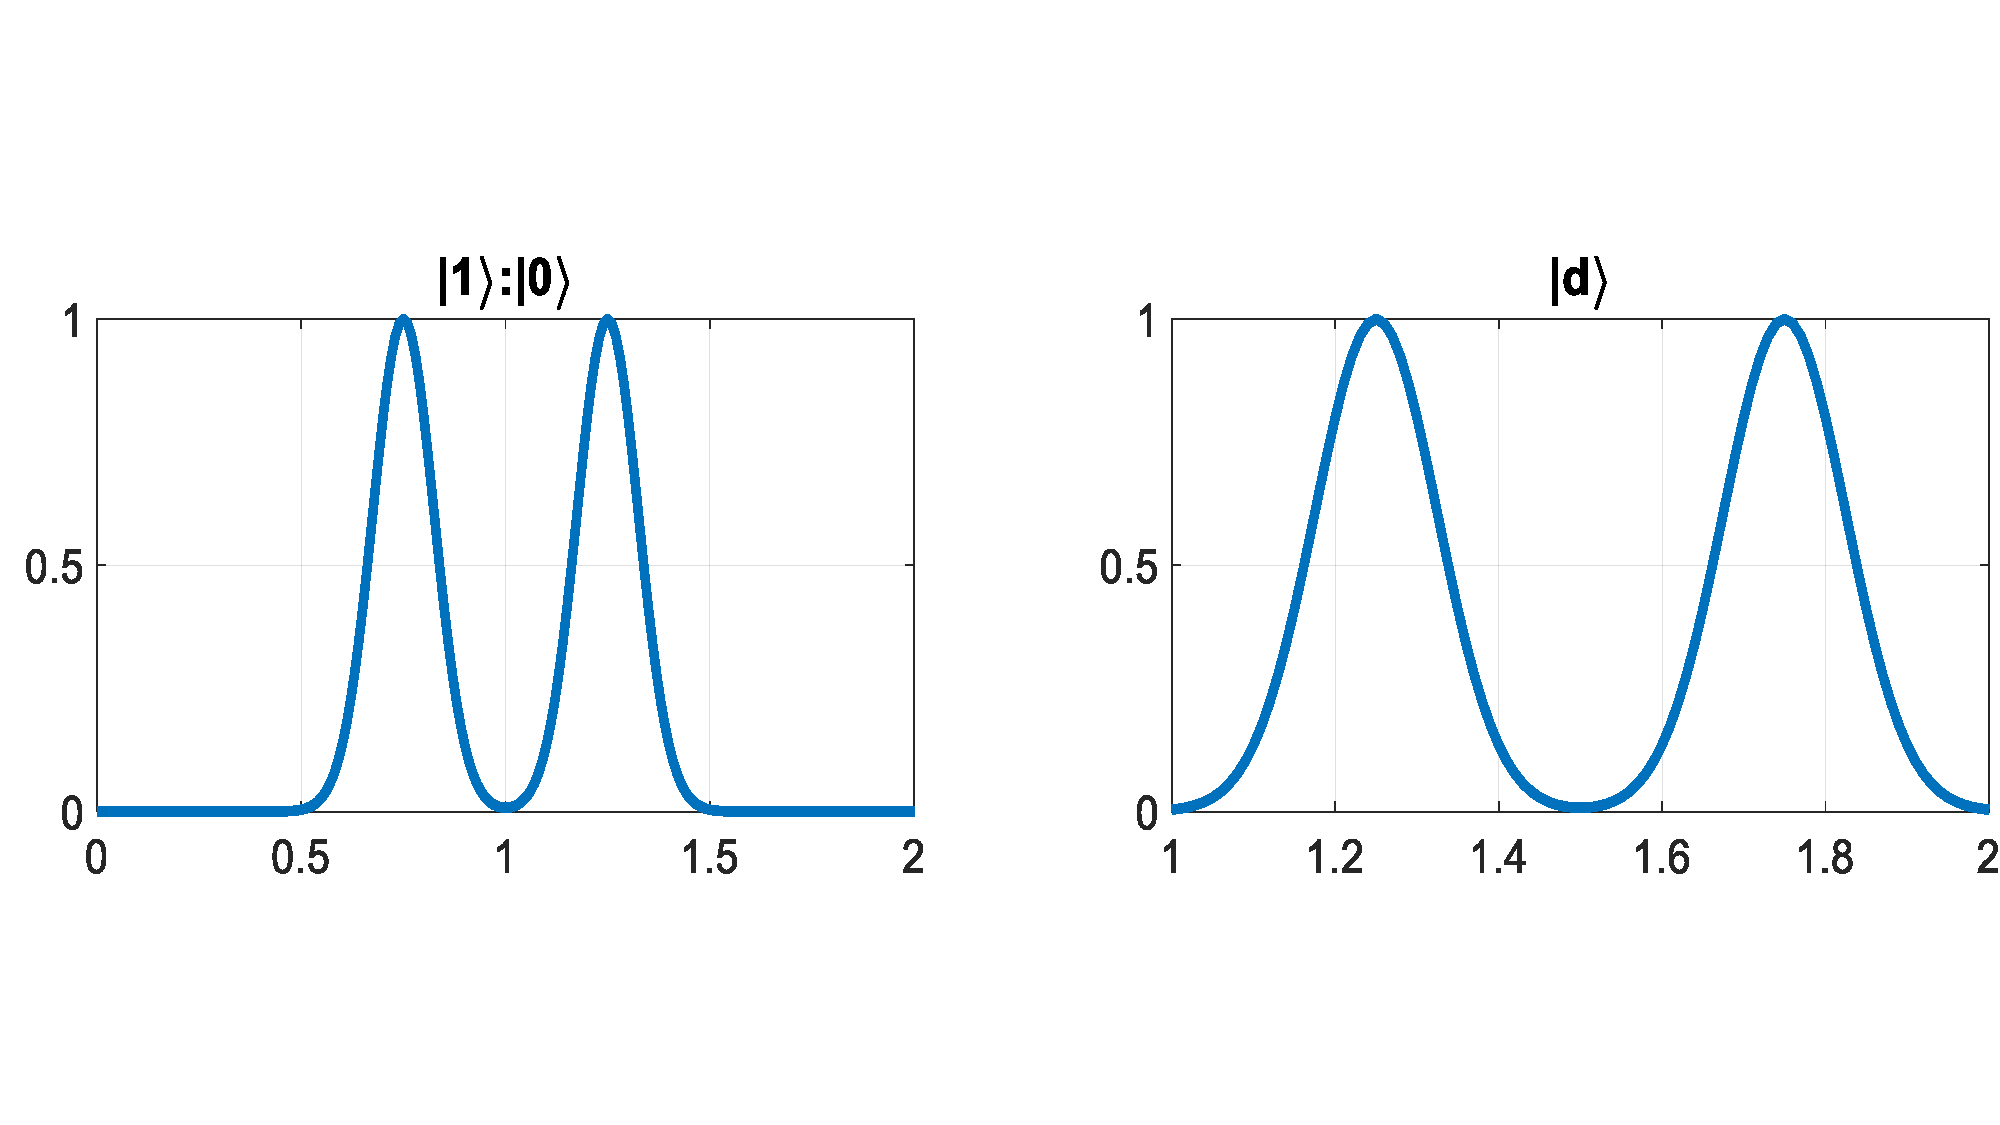
\includegraphics[width=0.4\linewidth]{./sdf/tq_76558_cow_protocol/slides/figures/S2.pdf}
\caption{Events where the $D_{M2}$ (constructive photon counter) clicks.}
\label{fig:dm2}
\end{figure}

\item [Step 3] Finally Alice tells Bob the times of Decoy, he removes them from the Data Line and checks if some of the $D_{M2}$ had fired during that time. This allows them to check for coherence in the same state.

If Eve were producing single photons, and seeding them in the right time bin, the main error that she would introduce was the lack of coherence.

\item [Step 4] Bob reveals all the other times that the $D_{M2}$ fired, Alice verifies if they all belong to the $|1\rangle:|0\rangle$ state. IF they don't belong means that someone introduced single photons generated from different lasers, what would, once again reveal the Eve in the line.

\item [Step 5] Bob reveals the times that he had a count in the data line, this allows Alice to delete from her part all the photons that were absorbed by the fibber.

\item [Step 6] On the final step they calculate QBER, check the number of the detections for every detector and if this two properties are within the expected they declared they run error correction and privacy amplification. At the end of this 6 step they have the key.

\end{itemize}

\subsection{Simulation Analysis}

For the simulation we wanted to see how robust is the protocol to the most basic attack possible, one intercept-resend all attack. On this attack Eve captures all the information, measures and then resend it to Bob. For representing the system used I have created a block diagram in Figure \ref{ref:bloc} and a representation like the one previously in Figure \ref{fig:E}.

\begin{figure}[h]
\centering
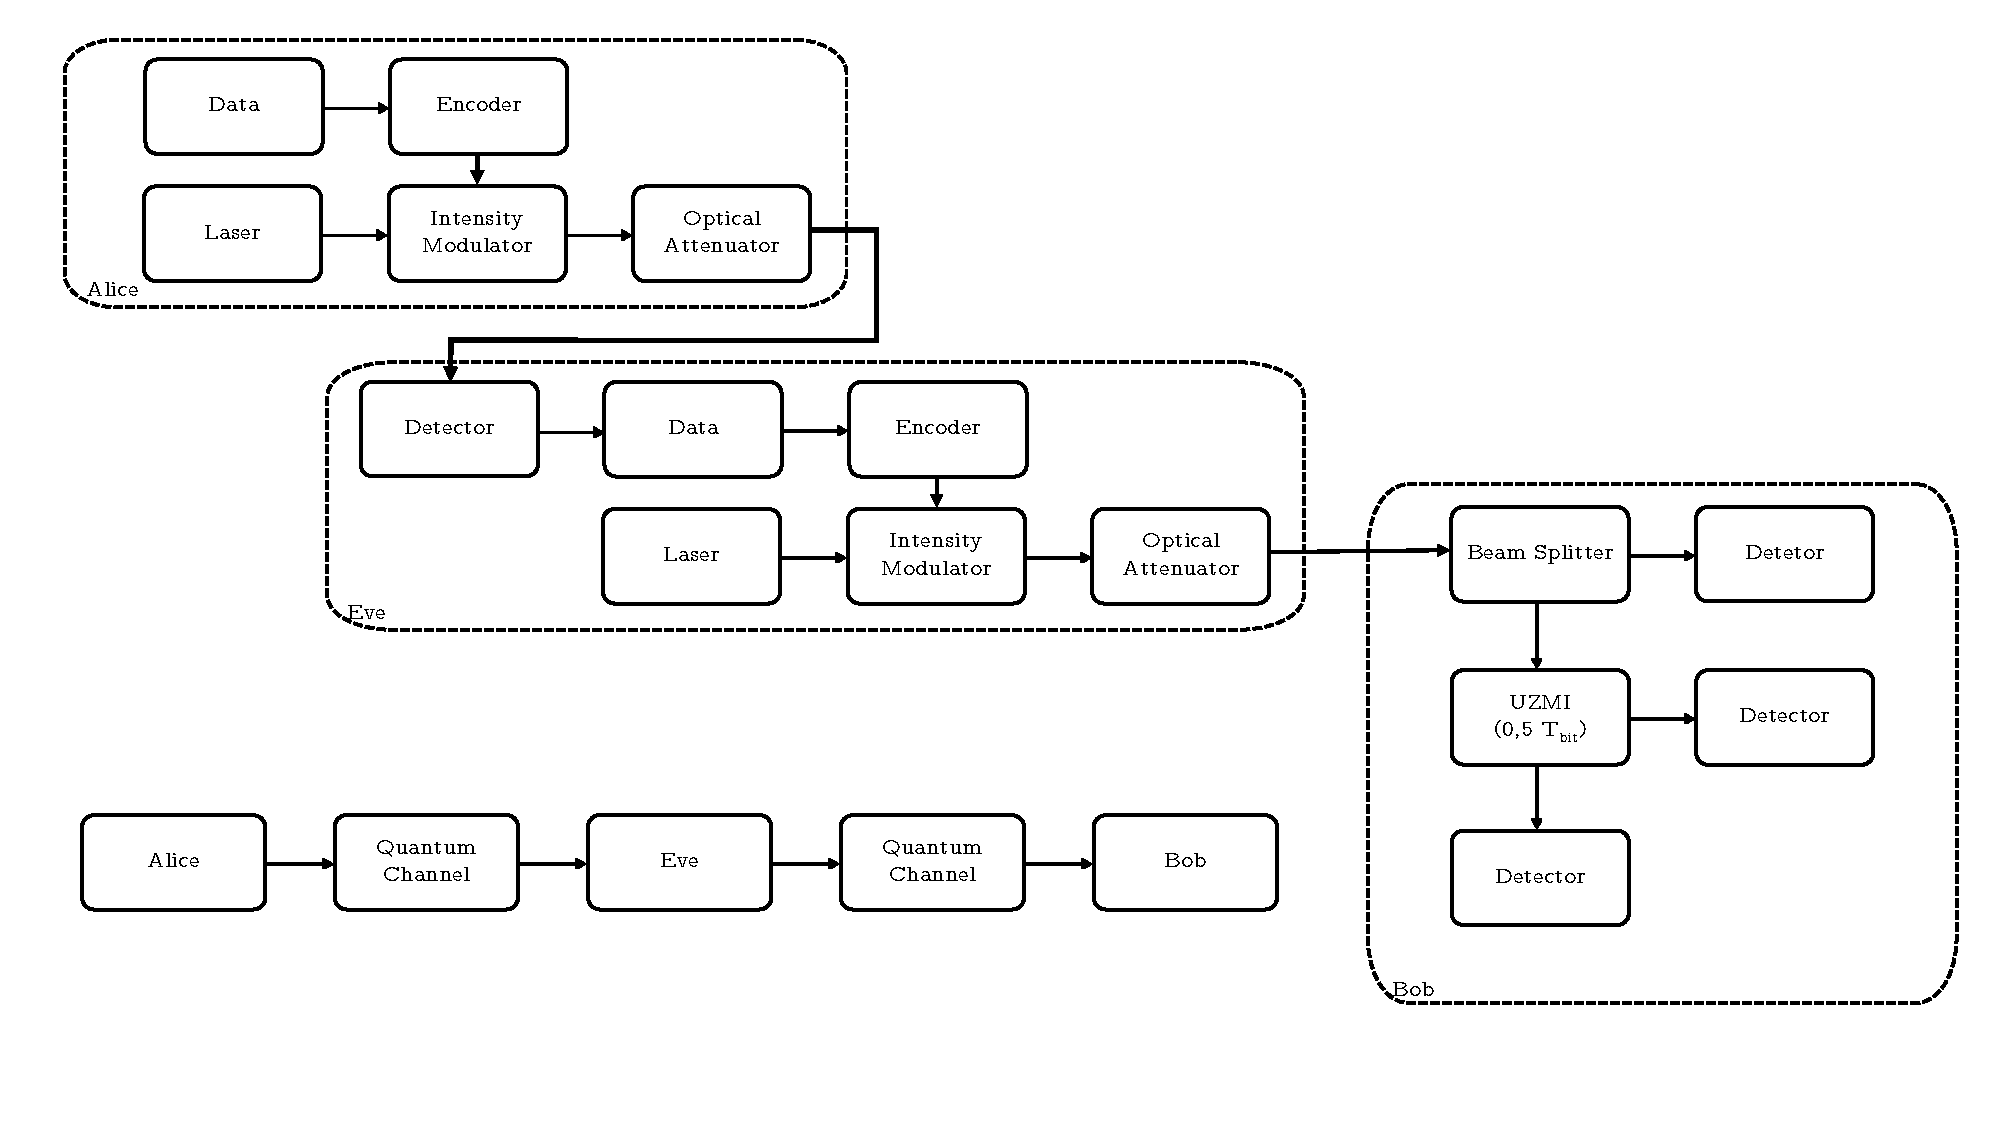
\includegraphics[width=0.4\linewidth]{./sdf/tq_76558_cow_protocol/slides/figures/Diagrama_de_blocos.pdf}
\caption{Block diagram for the basic IR attack.}
\label{fig:bloc}
\end{figure}

\begin{figure}[h]
\centering
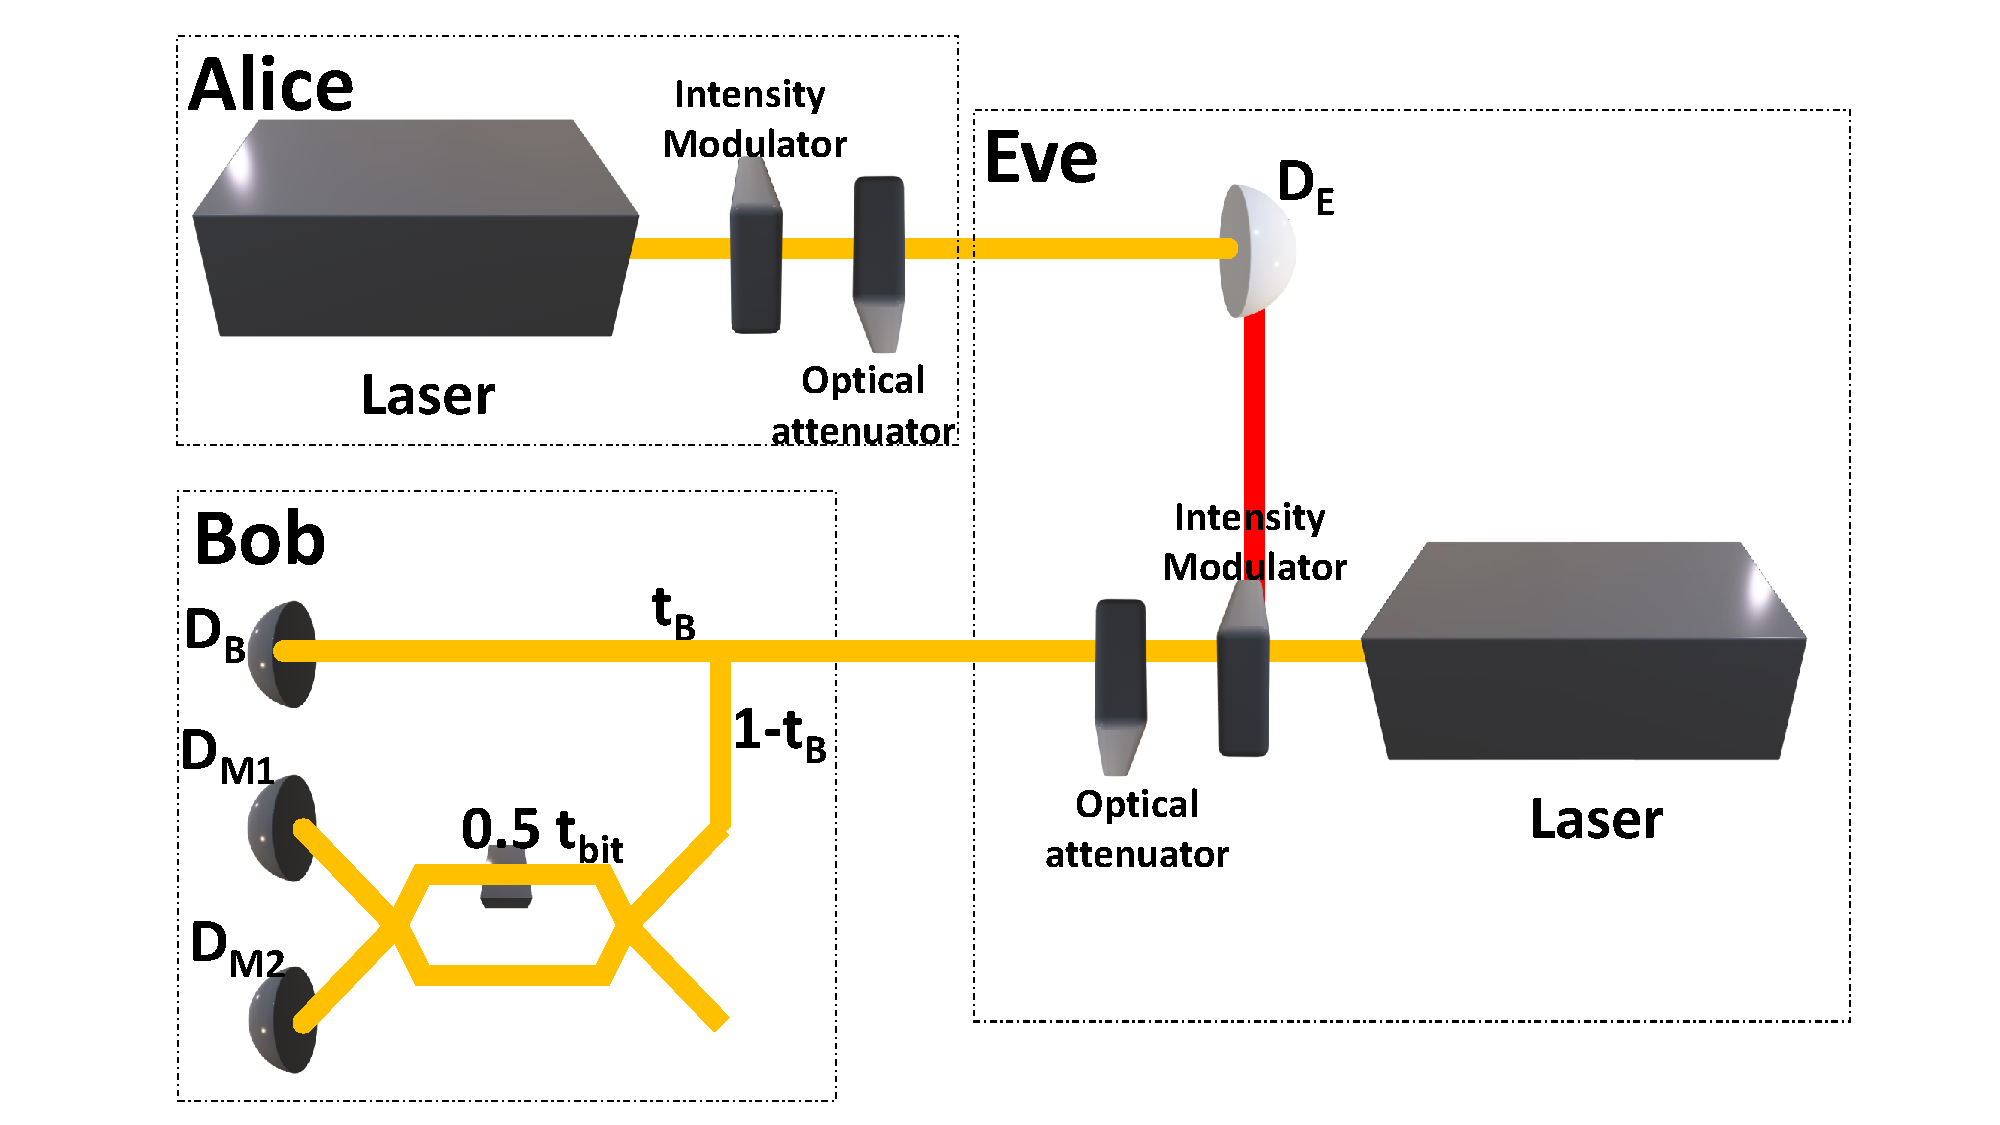
\includegraphics[width=0.4\linewidth]{./sdf/tq_76558_cow_protocol/slides/figures/E.pdf}
\caption{Simple scheme of the IR attack.}
\label{fig:E}
\end{figure}

For the simulation, I created a function ``Alice'' that generates a string with $10^7$ characters, every one of this characters has a $10 \%$ chance of being a ``d'' - representing a decoy state ($|d\rangle$), and half of the rest ($45 \%$) of being a ``0'' and the same probability of being a ``1'' - representing a zero state ($|0\rangle$) and a one state ($|1\rangle$) correspondent. The output of this function is a string with size $2\times10^7$ where all the states, have been replaced by ``1'' and ``0'' corresponding to the photons state and the vacuum state, the states where created using a Poisson distribution, but the completely empty states were removed. So this output variable has only the number of photons for every time bin, note that two time bin are needed for any state.

In this ``Alice'' function the decoy state only has near 1\% of probability of having photons in both pulses, most of the decoy states will only have photon in one of the pulses (90 \%).

$10^7$ logical bits in a fiber with 90 \% looses and with a attenuation of 0.1 from Alice is 1 second of the protocol working.

The second function called ``Eve'' captures all the information with her detector with a certain efficiency (the looses of the fibber were not simulated, wouldn't alter anything, would just make the simulation less efficient)  and then using a Poisson distribution generates the photons that sends to Bob in the same time bins that she has measured. The output of this function is once again a string with size $2\times10^7$, 

Finally I have created a function called ``Bob'' that would measure the incoming photons in 3 detectors, all of them with the same efficiency, and with probability of dark counts. Any photon that enter as input can either go for the data line (10 \% of the photons), or for the monitoring line (90 \%), in the data line they are simply registered as they come, and only one photon is needed, more photons do not alter anything, if he doesn't receive any photon, it can still register due to dark counts. If the photon goes to monitoring line, then he goes to another beamsplitter, this time with 50 \% probability for every outcome, in the first, he is delayed by half time_bin (if he doesn't interact in the next unit of time fires the $D_{M1}$), on the other outcome he interacts with the delayed photon, if there is no delayed photon, he fires the $D_{M1}$, if there is he fires the $D_{M2}$.

For this simulation in particular the difference between $D_{M1}$ and $D_{M2}$ doesn't alter anything, so I'm going to present the sum of both numbers, to reduce the unimportant information for this attack.

For the final function ``QBER'', a simple function that removes the decoy times from the Bob and Eve, due to the information from Alice and calculates QBER using a percentage of the total information that Bob got in the data Line (50 \% in this simulation).

I have run the simulation 200 times and then studied the average, the min and the max.

\subsection*{Inputs}

\begin{table}[hbt!]
\centering
\Large
\begin{tabular}{|c|c|}
\hline
\cellcolor[HTML]{005288}\color{white} Logical Bits from Alice & $10^{7}$\\ \hline
\cellcolor[HTML]{005288}\color{white} Probability of Decoy & 10 \% \\ \hline
\cellcolor[HTML]{005288}\color{white} Alice Attenuation & 0.1\\ \hline
\cellcolor[HTML]{005288}\color{white} Bob Detectors Efficiency  & 10 \% \\ \hline
\cellcolor[HTML]{005288}\color{white} Bob DarkCount Probability & $10^{-5}$ \\ \hline
\cellcolor[HTML]{005288}\color{white} Eve DarkCount Probability & $0$ \\ \hline
\cellcolor[HTML]{005288}\color{white} Average Over & 200 times\\ \hline
\cellcolor[HTML]{005288}\color{white} Percentage of the Key for QBER & 50 \% \\ \hline
\end{tabular}
\end{table}

\subsection*{Outputs}

This system outputs the following objects:

In a simulation without attack, and with this variables, the final information that Bob and Alice have is:

\begin{table}[hbt!]
\centering
\Large
\begin{tabular}{c|c|c|c|}
\cline{2-4}
\multicolumn{1}{l|}{} & \cellcolor[HTML]{005288}{\color[HTML]{FFFFFF} Min} & \cellcolor[HTML]{005288}{\color[HTML]{FFFFFF} Averag.} & \cellcolor[HTML]{005288}{\color[HTML]{FFFFFF} Max} \\ \hline
\multicolumn{1}{|c|}{\cellcolor[HTML]{005288}{\color[HTML]{FFFFFF} QBER}} & $9.9 \times 10^{-5}$ & 0.0001366 & 0.00018906 \\ \hline
\multicolumn{1}{|c|}{\cellcolor[HTML]{005288}{\color[HTML]{FFFFFF} $B_{M1}+B_{M2}$}} & 95294 & 96288 & 97069 \\ \hline
\multicolumn{1}{|c|}{\cellcolor[HTML]{005288}{\color[HTML]{FFFFFF} Key Length}} & 422730 & 423898 & 425281 \\ \hline
\end{tabular}
\end{table}

With the IR attack and using the Attenuation of Eve equal to 0.1, by changing the efficiency we get:

\begin{table}[hbt!]
\centering
\Large
\begin{tabular}{c|c|c|c|c|c|c|c|c|c|}
\cline{2-10}
 & \multicolumn{3}{c|}{\cellcolor[HTML]{005288}{\color[HTML]{FFFFFF} Eve Efficiency = 0.1}} & \multicolumn{3}{c|}{\cellcolor[HTML]{005288}{\color[HTML]{FFFFFF} Eve Efficiency = 0.5}} & \multicolumn{3}{c|}{\cellcolor[HTML]{005288}{\color[HTML]{FFFFFF} Eve Efficiency = 1}} \\ \cline{2-10} 
\multicolumn{1}{l|}{} & \cellcolor[HTML]{005288}{\color[HTML]{FFFFFF} Min} & \cellcolor[HTML]{005288}{\color[HTML]{FFFFFF} Averag.} & \cellcolor[HTML]{005288}{\color[HTML]{FFFFFF} Max} & \cellcolor[HTML]{005288}{\color[HTML]{FFFFFF} Min} & \cellcolor[HTML]{005288}{\color[HTML]{FFFFFF} Averag.} & \cellcolor[HTML]{005288}{\color[HTML]{FFFFFF} Max} & \cellcolor[HTML]{005288}{\color[HTML]{FFFFFF} Min} & \cellcolor[HTML]{005288}{\color[HTML]{FFFFFF} Averag.} & \cellcolor[HTML]{005288}{\color[HTML]{FFFFFF} Max} \\ \hline
\multicolumn{1}{|c|}{\cellcolor[HTML]{005288}{\color[HTML]{FFFFFF} QBER}} & 0.0020583 & 0.73014 & 1 & 0.0016881 & 0.22776 & 1 & 0.001729 & 0.0023946 & 0.00032631 \\ \hline
\multicolumn{1}{|c|}{\cellcolor[HTML]{005288}{\color[HTML]{FFFFFF} $B_{M1}+B_{M2}$}} & 0 & 1106 & 9261 & 0 & 4602 & 9383 & 8889 & 9173 & 9404 \\ \hline
\multicolumn{1}{|c|}{\cellcolor[HTML]{005288}{\color[HTML]{FFFFFF} Key Length}} & 85 & \cellcolor[HTML]{E5EAF4}4968 & 40642 & 91 &\cellcolor[HTML]{E5EAF4} 20361 & 40883 & 40034 &\cellcolor[HTML]{E5EAF4} 40438 & 40748 \\ \hline
\end{tabular}
\end{table}

With the IR attack and assuming that Eve has 100 \% efficiency. By altering the value of her attenuation we get:

\begin{table}[hbt!]
\centering
\Large
\begin{tabular}{c|c|c|c|c|c|c|}
\cline{2-7}
 & \multicolumn{3}{c|}{\cellcolor[HTML]{005288}{\color[HTML]{FFFFFF} Eve Attenuation = 1.101}} & \multicolumn{3}{c|}{\cellcolor[HTML]{005288}{\color[HTML]{FFFFFF} Eve Attenuation = 2}} \\ \cline{2-7} 
\multicolumn{1}{l|}{} & \cellcolor[HTML]{005288}{\color[HTML]{FFFFFF} Min} & \cellcolor[HTML]{005288}{\color[HTML]{FFFFFF} Averag.} & \cellcolor[HTML]{005288}{\color[HTML]{FFFFFF} Max} & \cellcolor[HTML]{005288}{\color[HTML]{FFFFFF} Min} & \cellcolor[HTML]{005288}{\color[HTML]{FFFFFF} Averag.} & \cellcolor[HTML]{005288}{\color[HTML]{FFFFFF} Max} \\ \hline
\multicolumn{1}{|c|}{\cellcolor[HTML]{005288}{\color[HTML]{FFFFFF} QBER}} & 0.00011775 & 0.00017323 & 0.00022875 & $6.21\times 10^{-5}$ & $8.93\times 10^{-5}$ & 0.00011472 \\ \hline
\multicolumn{1}{|c|}{\cellcolor[HTML]{005288}{\color[HTML]{FFFFFF} $B_{M1}+B_{M2}$}} & 99146 &\cellcolor[HTML]{E5EAF4} 100632 & 101557 & 181047 &\cellcolor[HTML]{E5EAF4} 182217 & 183986 \\ \hline
\multicolumn{1}{|c|}{\cellcolor[HTML]{005288}{\color[HTML]{FFFFFF} Key Length}} & 423756 & 424850 & 426440 & 739744 & 741841 & 743701 \\ \hline
\end{tabular}
\end{table}

\pagebreak
\subsection*{Conclusion - Simulation Results}
By having a efficiency lower than 100 \% Eve presence lowers the Key length.

And even if her efficiency was 100 \%, Eve presence still increases the sum ($B_{M1}+B_{M2}$) when the Key Length is the correct, and lowers the Key Length when the Sum ($B_{M1}+B_{M2}$) is correct.

\subsection{Comparative Analysis}

As we can see the Intercept Resend attack from Eve was a complete failure, even admitting a 100 \% and 0 \% probability of Dark Counts, she still changes the values that Bob obtains when she is not present, if she sends a different value of the Poisson distribution she alters the ratio of the Sum ($B_{M1}+B_{M2}$) by Key Length.


% bibliographic references for the section ----------------------------
\clearpage
\printbibliography[heading=subbibliography]
\end{refsection}
\addcontentsline{toc}{subsection}{Bibliography}
\cleardoublepage
% --------------------------------------------------------------------- 